%
\documentclass[12pt]{article}

% The usual packages
\usepackage{fullpage}
\usepackage{breakcites}
\usepackage{setspace}
\usepackage{endnotes}
\usepackage{float}
\usepackage{amsmath}
\usepackage{amsfonts}
\usepackage{amssymb}
\usepackage{rotating}
\usepackage{dcolumn}
\usepackage{longtable}
\usepackage{microtype}
\usepackage{graphicx}
\usepackage{hyperref}
%\usepackage[usenames,dvipsnames]{color}
\usepackage{url}
\usepackage{natbib}
\usepackage{framed}
\usepackage{epigraph}
\usepackage{lipsum}
\usepackage[font=small,labelfont=sc]{caption}
\restylefloat{table}
\bibpunct{(}{)}{;}{a}{}{,}

% Set paragraph spacing the way I like
\parskip=0pt
\parindent=20pt

% Define mathematical results
\newtheorem{lemma}{Lemma}
\newtheorem{proposition}{Proposition}
\newtheorem{theorem}{Theorem}
\newtheorem{claim}{Claim}
\newenvironment{proof}[1][Proof]{\begin{trivlist}
\item[\hskip \labelsep {\bfseries #1}]}{\end{trivlist}}
\newenvironment{definition}[1][Definition]{\begin{trivlist}
\item[\hskip \labelsep {\bfseries #1}]}{\end{trivlist}}
\newenvironment{example}[1][Example]{\begin{trivlist}
\item[\hskip \labelsep {\bfseries #1}]}{\end{trivlist}}
\newenvironment{remark}[1][Remark]{\begin{trivlist}
\item[\hskip \labelsep {\bfseries #1}]}{\end{trivlist}}

% Set up fonts the way I like
\usepackage{tgpagella}
\usepackage[T1]{fontenc}
\usepackage[bitstream-charter]{mathdesign}

%% Set up lists the way I like
% Redefine the first level
\renewcommand{\theenumi}{\arabic{enumi}.}
\renewcommand{\labelenumi}{\theenumi}
% Redefine the second level
\renewcommand{\theenumii}{\alph{enumii}.}
\renewcommand{\labelenumii}{\theenumii}
% Redefine the third level
\renewcommand{\theenumiii}{\roman{enumiii}.}
\renewcommand{\labelenumiii}{\theenumiii}
% Redefine the fourth level
\renewcommand{\theenumiv}{\Alph{enumiv}.}
\renewcommand{\labelenumiv}{\theenumiv}
% Eliminate spacing around lists
\usepackage{enumitem}
\setlist{nolistsep}

% Create footnote command so that my name
% has an asterisk rather than a one.
\long\def\symbolfootnote[#1]#2{\begingroup%
\def\thefootnote{\fnsymbol{footnote}}\footnote[#1]{#2}\endgroup}

% Create the colors I want
\usepackage{color}
\definecolor{darkred}{RGB}{100,0,0}

\hypersetup{
pdftitle={Substantive Importance and the Veil of Statistical Significance}, % title
pdfauthor={Kelly McCaskey and Carlisle Rainey}, % author
pdfkeywords={hypothesis testing} {confidence intervals} {substantive significance}
pdfnewwindow=true, % links in new window
colorlinks=true, % false: boxed links; true: colored links
linkcolor=black, % color of internal links
citecolor=black, % color of links to bibliography
filecolor=black, % color of file links
urlcolor=blue % color of external links
}

% enable comments in pdf
\newcommand{\kelly}[1]{\textcolor{blue}{#1}}
\newcommand{\carlisle}[1]{\textcolor{magenta}{#1}}

% April 6 Statistics Politics Policy submission
\begin{document}

\begin{center}
{\LARGE \textbf{Substantive Importance and the\\\vspace{2mm}Veil of Statistical Significance}\symbolfootnote[1]{We thank Lisa Hultman, Cindy Kam, Jacob Kathman, and Megan Shannon, and Elizabeth Zechmeister for making their data available to us. The analyses presented here were conducted with \texttt{R} 3.1.0. All data and computer code necessary to reproduce our paper and results are available at \href{https://github.com/carlislerainey/meaningful-inferences}{
github.com/carlislerainey/meaningful-inferences}.}}

\vspace{10mm}

Kelly McCaskey\symbolfootnote[2]{Kelly McCaskey is a Ph.D. student in the Department of Political Science, Texas A\&M University, 2010 Allen Building, College Station, TX, 77843 (\href{mailto:kellymccaskey@tamu.edu}{kellymccaskey@tamu.edu}).}

\vspace{3mm}

Carlisle Rainey\symbolfootnote[3]{Carlisle Rainey is Assistant Professor of Political Science, Texas A\&M University, 2010 Allen Building, College Station, TX, 77843 (\href{mailto:crainey@tamu.edu}{crainey@tamu.edu}).}
\end{center}

\vspace{10mm}

% Abstract
{\centerline{\textbf{Abstract}}}
\begin{quote}\noindent
Political science is gradually moving away from an exclusive focus on statistical significance and toward an emphasis on the magnitude and importance of effects. While we welcome this change, we argue that the current practice of ``magnitude-and-significance,'' in which researchers only interpret the magnitude of a statistically significant point estimate, barely improves the much-maligned ``sign-and-significance'' approach, in which researchers focus only on the statistical significance of an estimate. This exclusive focus on the point estimate hides the uncertainty behind a veil of statistical significance. Instead, we encourage researchers to explicitly account for uncertainty by interpreting the range of values contained in the confidence interval. Especially when making judgments about the importance of estimated effects, we advise researchers to make empirical claims if and only if those claims hold for the entire confidence interval.
 \end{quote}

% Add quote to first page
\epigraph{Far better an approximate answer to the \textit{right} question, which is often vague, than an exact answer to the \textit{wrong} question, which can always be made precise.}{\citet[pp. 13-14]{Tukey1962}}

% Remove page number from first page
\thispagestyle{empty}

% Start main text
\newpage
\doublespace

\section*{Introduction}

% This paragraph gives an overview of the paper. However, I'm not sure that it is needed, since it largely duplicates the abstract. Instead, perhaps we should lead with examples of claims about substantive significance?
Recent work in political science encourages researchers to move beyond statistical significance (i.e., null hypothesis significance testing) and focus on the substantive or political importance of the effect (e.g., \citealt{KingTomzWittenberg2000}; \citealt{HanmerKalkan2013}; \citealt{EsareyDanneman2014}; and \citealt{Gross2014}). The current practice in political science argues for substantive importance by interpreting the magnitude of statistically significant point estimates. If the estimate is substantively large, then the researcher concludes the effect is ``substantively and statistically significant.'' However, this approach is not convincing. In this paper, we show that focusing \emph{only} on the magnitude of the estimated effect retains many of the flaws associated with focusing \emph{only} on statistical significance. Instead, researchers should account for the uncertainty of the estimates when arguing for substantive significance by interpreting not only the point estimate but also the range of values in the confidence interval. This idea is not new (e.g., \citealt{Achen1982}, \citealt{Gross2014}, and \citealt{Rainey2014a}), but it has not become common practice. 

Our aims are twofold. First, we explain the problem with the current practice, and second, we explain how researchers can use confidence intervals to more clearly evaluate claims that effects are large enough to matter for politics and policy. Our key point is that researchers should interpret the range of values contained in their confidence intervals and, conversely, avoid making claims that are not consistent with the range of values in their confidence intervals.

% There are three questions that political scientists care about.
We contend that the best empirical political science concerns itself with the (1) direction, (2) magnitude, and (3) substantive importance of the effects of interest. Each component requires increasing levels of analysis and substantive interpretation and each receives decreasing levels of attention. Virtually every research article in empirical political science makes an argument about the direction of the effect using a significance test. Almost all of these articles report some measure of effect size, if only a table of regression coefficients. 

% The third is usually not.
However, judgments about the importance of the effect are often missing. To get a sense of how often researchers address substantive importance (i.e., Are the effects large enough to care about?), we reviewed all articles published in the \textit{American Political Science Review} and the \textit{American Journal of Political Science} from 2011 to 2013.\footnote{To do this, we read the 316 articles published in the range of years and coded whether or not each was an empirical study. Of those that were empirical, if the author made the claim that the estimate was large because of some theory-based reason, the article was coded as having made an explicit argument about the substantive nature of the study's results.}  Of the 316 total articles, 73\% present empirical analyses. Of this 73\%, only about half contain a judgment about the substantive importance of the estimated effect. Furthermore, of the articles that judge the substantive importance of their results, only 17\% actually make an explicit argument that the estimates are substantively large.

% Overview of the paper
We begin by elaborating on the questions that political scientists typically ask about effects and explain the typical approaches to answering these questions. We then provide an overview of the much-maligned sign-and-significance approach and the current best practice of magnitude-and-significance. In addition, we explain why the magnitude-and-significance approach is only a small improvement over the sign-and-significance approach. As an alternative, we suggest that researchers focus on the range of values contained in the confidence interval and avoid focusing exclusively on the point estimate. We conclude with empirical examples that highlight the consequences of substantively interpreting the range of effects that are consistent with the data.

\section*{What We Want To Know}

% What we mean by "an effect."
Most empirical research in political science focuses on estimating the effect of an explanatory variable on the expected value of an outcome of interest. To fix ideas, we denote the outcome variable $y$ and the explanatory variable $x$ and let $E(y | x) = f(x)$. For concreteness, define the ``effect'' or ``quantity of interest'' $\Delta$ as the difference between the average outcome when $x$ takes on a substantively meaningful high value and low value, so that $\Delta = E(y | x = x_{hi}) - E(y | x = x_{lo}) = f(x_{hi}) - f(x_{lo})$. Empirical work usually focuses on three fundamental questions about the effect of the explanatory variable on the outcome. We explain each, in turn, in the following sections.

\begin{enumerate}
\item What is the direction of the effect?
\item How large is the effect?
\item Is the effect substantively important?
\end{enumerate}

\subsection*{Direction}

% Orient the reader to the direction question
The first question that empirical research usually attempts to answer is the direction of the effect. In other words, is the effect positive or negative?\footnote{Some research argues theoretically and empirically for ``no effect'' or ``a negligible effect'' (e.g., \citealt{KamPalmer2008}, though see \citealt{Rainey2014a}), but most hypotheses posit the direction of an effect.} 

% Provide the details of the direction question
For clarity, suppose that the researcher offers a directional research hypothesis, suggesting that an effect of interest is positive. To evaluate the evidence for her hypothesis, the researcher usually calculates a $p$-value--the maximum probability of obtaining hypothetical data at least as extreme as the observed data if the null hypothesis were true. If this $p$-value is sufficiently small (by convention, less than 0.05), then the researcher concludes that the effect is positive. However, if the $p$-value is not sufficiently small, then the researcher declares that the data do not offer compelling evidence against the null hypothesis and notes that the direction of the effect remains uncertain.\footnote{However, some research takes a $p$-value greater than 0.05 as evidence \textit{in favor of} the null hypothesis \citep{Rainey2014a}. We prefer to interpret a lack of statistical significance as ambiguous evidence from which the researcher can make no claim (i.e., the effect might be negative or positive).}

% Three things to note about arguments for direction.
%There are three features of arguments for direction to make note of. First, this style of argumentation is ubiquitous in political science. It is extremely rare to find empirical research in political science that does not perform a hypothesis test of some sort. Each empirical study published in the \textit{APSR} and \textit{AJPS} from 2011 to 2013 performs some type of hypothesis test. Second, this approach is compelling--not because it argues that the observed data are consistent with the researcher's claim--but because the data are inconsistent with other claims. Third, this argument for the direction of the effect explicitly accounts for the uncertainty of the estimated effect. If the uncertainty is large relative to the magnitude of the estimate then the researcher cannot (and usually does not) make confident claims about the direction of the effect of interest. However, if the uncertainty is small relative to the size of the estimated effect, then the researcher can draw confident conclusions about the direction of the effect. 

\subsection*{Magnitude}

% Orient the reader toward the magnitude question
However, recent methodological work points out that empirical research should go beyond estimating the direction of the effect and emphasize the size or magnitude of the effect as well (\citealt{KingTomzWittenberg2000}; \citealt{HanmerKalkan2013}; \citealt{Gross2014}). In discussing how scholars might interpret a model of the effects of education on income, \citet[p. 348]{KingTomzWittenberg2000} write:

\begin{quote}
Bad interpretations are substantively ambiguous and filled with methodological jargon: ``the coefficient on education was statistically significant at the 0.05 level.'' Descriptions like this are very common in social science, but students, public officials, and scholars should not need to understand phrases like ``coefficient,'' ``statistically significant,'' and ``the 0.05 level'' to learn from the research. Moreover, even statistically savvy readers should complain that the sentences does not convey the key quantity of interest: how much higher the starting salary would be if the student attended college for an extra year.
\end{quote}

% However, the idea that magnitude is important has been around a while
The emphasis on effect magnitude is hardly a new idea. Commenting on the consequences of Fisher's null hypothesis significance test, \citet[p. 32]{Yates1951} writes: ``[I]t has caused scientific workers to pay undue attention to the results of the tests of significance they perform on their data, particularly data derived from experiments, and too little to the estimates of the magnitude of the effects they are investigating.'' Yates continues: 

\begin{quote}
Tests of significance are preliminary or ancillary. The emphasis on tests of significance, and the consideration of the results of each experiment in isolation, have had the unfortunate consequence that scientific works have regarded the execution of a test of significance on an experiment as the ultimate objective. Results are significant or not significant and that is the end of it (p. 33).
\end{quote}

% Substantively interpretable measures of magnitude are easy.
But \cite{KingTomzWittenberg2000} show that computing an interpretable measure of effect magnitude is not always straightforward. Only some statistical models have naturally interpretable parameters. For example, a simple difference-in-means or normal-linear model has directly interpretable coefficients as long as the scales of the variables are reasonable and the model does not include non-linear or product terms. Outside of this atypical situation, however, the researcher must do additional work to estimate a substantively meaningful quantity of interest. Fortunately, recent conceptual work (\citealt{KingTomzWittenberg2000}; \citealt{BerryDeMerittEsarey2010}; and \citealt{HanmerKalkan2013}) and software development (\citealt{TomzWittenbergKing2003}; and \citealt{ImaiKingLau2007}) empower political scientists to move beyond a simple ``sign-and-significance'' approach and also present substantively meaningful measures of effect magnitude. 

\subsection*{Importance}

% Orient the reader to the question of importance
Researchers ultimately want to move beyond the simple presentation of effect magnitude and make a judgment about the meaningfulness of the effects. Is the effect large or small? Is it politically important? Is it relevant for policy? Is it scientifically important? Is it large enough to matter? \citet[p. 264]{HanmerKalkan2013} write: ``[W]e take it as given that understanding whether the relationship is substantively significant, rather than just statistically significant, is the ultimate goal, as it is a necessary part of evaluating one's theory.''

As \cite{Rainey2014a} notes, political scientists should not insist on hard and fast rules for judging the effects that are and are not substantively meaningful.\footnote{We should note, though, that such rules of thumb have been presented, see \cite{Glass1976} and \cite{Cohen1992}, but these rules are usually proposed with caution.} Instead, we must insist that substantive scholars making substantive claims about politics also make substantive judgments about the importance of their effects. \citet[pp. 82-83]{Thompson2001} writes that ``if people interpreted effect sizes with the same rigidity that $\alpha = 0.05$ has been used in statistical testing, we would merely be being stupid in another metric.'' \cite{Kirk1996} suggests that this judgment is ``influenced by a variety of factors, including the researcher's value system, societal concerns, assessment of costs and benefits, and so on.'' Similarly, \citet[p. 30]{Thompson2002} writes: 

\begin{quote}
The existence of effect size benchmarks should not justify abrogating the responsibility for arguing for effect import in the specific context of a given study. It is not necessary to have universal benchmarks regarding what effect sizes may be deemed noteworthy. The reader with a value system widely different than that of an author might reasonably disagree with the author about whether the effect size is noteworthy and then simply ignore the study.
\end{quote}

Substantive judgments about effect sizes require a large initial investment of careful thought, and this judgment demands subjectivity (see \citealt{Rainey2014a}). However, because this subjective judgment is transparent, readers are free to reject the author's judgment and substitute their own. Further, ``automatic'' and ``objective'' procedures are not always (or perhaps usually) desirable.\footnote{Formal hypothesis tests and judgments about substantive importance are qualitatively different decisions and have different strengths and weaknesses. Estimation and hypothesis tests are relatively automatic and ``objective,'' but not transparent. Researchers do not fit one model and report the single $p$-value. Instead they fit many models and report the one that ``makes most sense'' in light of their approach, theoretical model, normative concerns, and the results of the model (\citealt{GerberMalhotra2008}; \citealt{SimmonsNelsonSimonsohn2011}; \citealt{Francis2013}; \citealt{SimmonsNelsonSimonsohn2014}; and \citealt{EsareyWu2014}; see also \citealt{GelmanLoken2014}).} Substantive scholars making substantive points about politics must not be prohibited from making substantive judgments. Instead, they must be \emph{encouraged} to do so \citep{Achen1982}. Indeed, \citet[p. 755]{Kirk1996} writes:

\begin{quote}
Researchers have an obligation to make this kind of judgment. No one is in a better position than the researcher who collected and analyzed the data to decide whether or not the results are trivial. It is a curious anomaly that researchers are trusted to make a variety of complex decisions in the design and execution of an experiment, but in the name of objectivity, they are not expected or even encouraged to decide whether data are practically significant.
\end{quote}

% one example of a claim of importance
For example, \citet[p. 711]{KingZeng2001} claim that, ``if a collection of 300,000 dyads shows a 0.001 increase in the probability of war, the finding is catastrophically important because it represents about three hundred additional wars and a massive loss of human life'' (emphasis ours). In another example, \citet[p. 317]{HetheringtonSuhay2011} note that 
\begin{quote}
When we fixed trust at its minimum, the predicted probability that our typical respondent thought Iraq was worth the cost was only 0.33; we would classify him as not believing Iraq was worth the cost. If we increase political trust to its maximum, however, the predicted probability more than doubles to 0.72, a 39 percentage point increase. This is substantively important because, with trust at its maximum, our typical respondent believes Iraq was worth the cost.
\end{quote}
This raises three questions about the process of judging an effect to be important for politics and/or policy.
\begin{enumerate}
\item What is the current practice for making these judgments?
\item Is this practice compelling?
\item If not, what might serve as a better approach?
\end{enumerate}
\noindent We now turn to these questions.

\section*{Current Practices in Reasoning About Effect Importance}

% Brief summary of the sign-and-significance approach
%Two current practices dominate the way that researchers make statistical arguments for substantive importance. We show that both of these approaches are flawed and we argue for a third, improved method. 

%First, researchers might deem any statistically significant result as an important one. We refer to this as the ``sign-and-significance'' approach in which researchers simply note the sign of an effect and claim it is statistically significant. This approach incorrectly interprets the $p$-value as a measure of magnitude or importance, though perhaps only implicitly.

% Brief summary of the magnitude-and-significance approach
%The second practice, which is more common in political science, is to interpret the magnitude without explicitly accounting for the uncertainty of the estimate. We refer to this as the ``magnitude-and-significance'' approach in which researchers first check that an effect is statistically significant and then interpret the magnitude of the estimate. While the magnitude-and-significance approach is no doubt and improvement on the sign-and-significance approach, we show that it retains many of its flaws.

% Brief summary of the explicit-test approach
%As an alternative, we suggest that researchers explicitly account for uncertainty when arguing for meaningful effects by simply focusing on confidence intervals rather than point estimates \citep{Gross2014}. Researchers must simply interpret the range of values that lie within the confidence interval and avoid drawing strong conclusions from the point estimate that are not consistent with the range of values in the confidence interval.

\subsection*{Sign-and-Significance}

% Overview of the SS approach
Using the sign-and-significance approach, researchers declare an effect important if and only if the effect is statistically significant. That is, researchers simply test whether the effect is greater than (or less than) zero. If they reject the null hypothesis (e.g., $p < 0.05$), then they declare, or perhaps subtly imply, the effect to be substantively meaningful. While this approach is not commonly employed in political science research, it is important to highlight because its shortcomings are well understood \citep{Gill1999}.

% The problems with the SS approach
The much maligned (e.g., \citealt{Cohen1990}, \citealt{Gill1999}, \citealt{HillJones2014}, and \citealt{Gross2014}) sign-and-significance approach emphasizes $p$-values, but a minuscule $p$-value does not imply a large or important effect. The $p$-value depends on both the sample size and the effect size. It is true that the $p$-value gets smaller as the effect size under investigation increases. However, the $p$-value also decreases as the sample size increases, which is unrelated to the effect size. While political scientists often describe estimates as ``highly significant'' or ``very significant,'' this implies (or tempts readers to conclude) that an effect is large or important. But ``very significant'' (e.g., $p < 0.001$) might simply mean that the researcher has a large sample. Even if the researcher finds statistically significant results with a small sample, the small $p$-value only indicates that the effect size is large relative to the uncertainty. It says nothing about the size of the estimate relative to some standard of substantive importance. With a very small $p$-value (e.g., $p < 0.001$), substantive experts might judge the effect to be large, moderate, small, or even negligible. Experts might call some of these effects important, somewhat important, slightly important, or not at all important. The $p$-value is indirectly related to substantive significance at best.

\subsection*{Magnitude-and-Significance}

% Overview of the MS approach
Fortunately, political science has moved beyond the sign-and-significance approach. Instead, most research now adopts the ``magnitude-and-significance'' approach, in which the researcher takes the following steps: 

\begin{enumerate}
\item Computes substantively interpretable estimate of the effect of interest, such as a first difference.
\item Tests whether this estimate is statistically significant.
\item If so, makes a judgment about whether the magnitude of the estimate is substantively important.
\end{enumerate}

% Example 1
For example, \cite{TomzWeeks2013} discuss the results of their experiment on attitudes about conflict.

\begin{quote}
Citizens in both countries were much less willing to attack another democracy than to attack an otherwise equivalent autocracy. Approximately 34.2\% of respondents in the U.K. supported a military strike when the country was not a democracy versus 20.9\% when the country was a democracy. Thus, democracy reduced support for a military strike by more than 13 percentage points, with a 95\% confidence interval of 19.6 to 6.9. The baseline level of militarism was much higher in the United States, where at least half the respondents wanted to strike an autocracy. Nonetheless, democracy exerted a similarly large effect in the United States: The between-subjects and within-subject estimates concurred that democracy reduced enthusiasm for a military strike by about 11.5 percentage points. In both countries, democracy produced \emph{substantively large and statistically significant} effects on preferences (p. 854-855, emphasis ours).
\end{quote}

% Example 2
\cite{GerberHopkins2011} discuss their regression model.

\begin{quote}
The first model indicates that all else equal, a city where the Democrat just wins the mayoralty should expect its spending on police to drop by 2.3 percentage points three fiscal years later. This result is \emph{statistically significant}, with a 95\% confidence interval that runs from 0.5 percentage points to 4.0 percentage points. It is \emph{substantively large as well}, as it reflects a spending shift of 1.2 standard deviations in terms of the dependent variable (p. 333, emphasis ours).
\end{quote}

%% Example 3
%\cite{AnsolabehereJones2010} discuss the coefficients of their regression model.
%
%\begin{quote}
%The regression results in [their] Table 3 show that a Representative's actual roll-call votes strongly predict respondents' beliefs about the Representative's votes. The coefficients for both 2005 and 2006 are \emph{substantively large} (approximately 0.3) \emph{and statistically significant} (p. 588, emphasis ours). 
%\end{quote}

% Problems with the MS approach
Notice that the magnitude-and-significance approach places uncertainty behind the veil of statistical significance. The analysis appears to take account of uncertainty with a significance test, but the significance test does not correspond to the substantive claim. The significance test does not illuminate the uncertainty--it acts as a veil that conceals the uncertainty. As a result, the magnitude-and-significance approach tempts researchers to do the following:

\begin{enumerate}
\item Treat all statistically significant and substantively large estimates similarly, drawing no distinction between large, imprecise estimates and large, precise estimates.
\item Treat ``barely significant'' large estimates and ``almost significant'' large estimates quite differently, drawing a strong distinction between two similar estimates with similar uncertainty.
\item Treat all results that are not statistically significant similarly, drawing no distinction between large, imprecise estimates and small, precise estimates (see Rainey 2014).
\end{enumerate}

% Frequency properties
What can we say about the consequences of the magnitude-and-significance approach? In particular, what can we say about its frequentist properties? Consider the ideal properties of a test. Suppose the researcher wishes to evaluate the theoretical prediction that a variable of interest has a positive, substantively large effect. That is, she posits the research hypothesis $H_r: \Delta > m$, where $m$ represents the cutoff between meaningful and negligible effects (see \citealt{Rainey2014a}). $H_r$ implies the null hypothesis $H_0: \Delta \leq m$. Following conventional standard, we prefer (and readers expect) the researcher to use a procedure such that when the null hypothesis is true, the researcher rarely claims support for the research hypothesis. Formally, this requires that, for all $\Delta \leq m$, the probability of accepting the research hypothesis $H_r: \Delta > m$ (or rejecting the null hypothesis $H_0: \Delta \leq m$) must be sufficiently small, conventionally less than or equal to 0.05. We refer to a test that meets this requirement as a size-0.05 test.

The magnitude-and-significance approach is not a size-0.05 test of the research hypothesis that a variable has a meaningful effect. Under the null hypothesis, the probability of accepting the research hypothesis might be as large as 0.50--a coin flip. Further, this can easily occur in actual analyses. For example, suppose an estimator $\hat{\Delta} \sim N(\Delta, \sigma^2)$ with standard error $\sigma < \frac{m}{1.64}$. If $\Delta = m$ (i.e., the null hypothesis holds), then the probability that $\hat{\Delta} > \Delta$ equals 0.50 and each of these estimates is also statistically significant. That is, even when the effect is actually negligible, the researcher using the magnitude-and-significance approach risks claiming ``substantive significance'' much too often.

% Introduce the example cis figure
Consider, for example, the hypothetical studies presented in Figure \ref{fig:example-cis}. If we are interested in substantive significance and consider 0.25 as the cutoff between meaningful and negligible effects, then only one study, Study A, seems to offer strong evidence for a substantively meaningful effect. Studies B and C offer ambiguous evidence for a meaningful effect and Studies D and E offer evidence \emph{against} a meaningful effect.

\begin{figure}[H]
\begin{center}
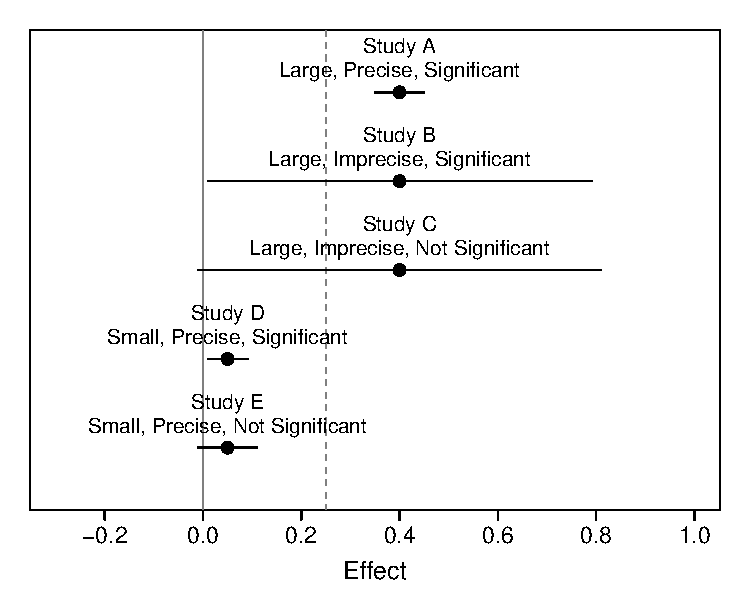
\includegraphics[scale = .8]{figs/example-cis.pdf}
\caption{This figure provides several hypothetical studies to illustrate several points about arguments for substantive significance. Notice that Study A offers compelling evidence for a meaningful effect, Studies B and C are consistent with both small and large effects, and Studies D and E offer evidence \emph{against} meaningful effects. However, the current practice in political science of magnitude and significance treats Studies A and B similarly, Studies B and C \emph{differently}, and Studies C and E similarly. Table \ref{tab:example-cis} compares the interpretations from both the sign-and-significance and magnitude-and-significance approaches with the intuitive meaning.}\label{fig:example-cis}
\end{center}
\end{figure}

% It treats studies A and B the same
Although only Study A offers compelling evidence for a meaningful effect, the magnitude-and-significance approach suggests that Studies A and B offer similar evidence for a substantively meaningful effect as well, because both are ``statistically significant and substantively large.''  Yet these studies do not offer similar evidence for a meaningful effect. Study A is \textit{only} consistent with a meaningful effect. Study B, on the other hand, is also consistent with small, negligible effects.

% It treats B and C differently
In fact, the amount of evidence for a meaningful effect offered by Study B is similar to that offered by Study C--both studies are consistent with both large and small effects. Nevertheless, the magnitude-and-significance approach treats these studies \emph{differently}. The magnitude-and-significance approach concludes from Study B that the effect is ``positive, significant, and substantively meaningful''  and from Study C that the effect is ``not statistically significant.''

% It treats C and E the same
The magnitude-and-significance approach also treats Studies C and E similarly because both estimates are ``not statistically significant.'' However, Study C is consistent with large \emph{and} small effects. Study E, in contrast, is consistent with \emph{only} small effects.

% The MS approach has many of the same problems as the SS approach.
The only actual improvement of the magnitude-and-significance approach over the much maligned sign-and-significance approach is that the magnitude-and-significance approach manages to distinguish between Study A and Study D. Other than that, both of these approaches treat Study A and B similarly, Studies B and C differently, and Studies C and E similarly. From our perspective, these are all inferential errors. Table \ref{tab:example-cis} shows the interpretation from each approach compared with an ``intuitive interpretation'' based on a simple inspection of the confidence intervals. Pay particular attention to the similarity of the errors made by the dismissed sign-and-significance approach and the current practice of magnitude-and-significance.

\singlespace
\renewcommand{\arraystretch}{1.5}
\begin{table}[H]
\begin{center}
\begin{scriptsize}
\begin{tabular}{|>{\centering\arraybackslash}m{.5in}>{\centering\arraybackslash}m{1.75in}>{\centering\arraybackslash}m{1.75in}>{\centering\arraybackslash}
m{1.75in}|}
\hline
Study & Sign-and-Significance Method & Magnitude-and-Significance & Intuitive Interpretation\\ 
\hline
Study A & ``positive and significant'' & ``positive, significant, and substantively large'' & ``We have strong evidence for a large, substantively meaningful effect.''\\
Study B & ``positive and significant'' & ``positive, significant, and substantively large'' & ``We have only weak evidence for a large, substantively meaningful effect, because the data are also consistent with negligible effects near zero.''\\
Study C & ``not statistically significant'' & ``not statistically significant'' & ``We have only weak evidence for a large, substantively meaningful effect, because the data are also consistent with negligible effects near zero.''\\
Study D & ``positive and significant'' & ``positive and significant, but substantively small' & ``We have strong evidence against a substantively meaningful effect.''\\
Study E & ``not statistically significant'' & ``not statistically significant'' & ``We have strong evidence against a substantively meaningful effect.''\\
\hline
\end{tabular}\caption{This table compares the interpretations of the results in Figure \ref{fig:example-cis} using the sign-and-significance and the magnitude-and-significance approaches to the intuitive meaning of the confidence intervals. Notice that the much maligned sign-and-significance approach and the magnitude-and-significant approach only differ in their interpretations of Studies D and E. Both approaches deviate substantially from the intuitive interpretation based on the confidence intervals.}\label{tab:example-cis}
\end{scriptsize}
\end{center}
\end{table}
\doublespace

% We need to be consistent with the standard of evidence
It is important to apply similar standards of evidence to arguments for positive (or negative) effects and arguments for \emph{meaningfully} positive (or negative) effects. The usual logic of hypothesis testing requires that the researcher declare that an effect is positive (or negative) if and only if the evidence overwhelmingly points toward a positive (or negative) effect. Similarly, researchers should not declare a positive estimate to be substantively meaningful simply because it is inconsistent with negative effects and the point estimate lies above some threshold. A consistent standard of evidence requires that researchers declare an effect to be substantively meaningful if and only if it is inconsistent with negligible effects.

\subsection*{Confidence Intervals}

% Overview
As one solution to the problem, \cite{Gross2014} presents the formal PASS test.\footnote{We recommend reading Gross (2014) as a companion paper. Our articles offer different perspectives, but make similar suggestions to substantive researchers.} Using the PASS test, researchers specify a pre-chosen value (that we denote as) $m$ that represents the cutoff between meaningful and negligible effects. Values larger than $m$ are thought to be substantively important and values smaller than $m$ are thought to be substantively \textit{un}important. This enables the researcher to specify and test a hypothesis $H_r: \Delta > m$ that corresponds to the substantive claim.

While this formal hypothesis testing framework is sometimes clear and convenient, confidence intervals offer even more information and are easier for researchers (and readers) to interpret. There is a one-to-one correspondence between a hypothesis test and a confidence interval. Specifically, a 90\% confidence interval contains only values greater than $m$ if and only if a size-0.05 hypothesis test rejects the null hypothesis that the effect is less than or equal to $m$. Therefore, if the 90\% confidence interval contains only large, meaningful effects, then the researcher can confidently reject the null hypothesis of a small, negligible effect. However, if the 90\% confidence interval contains effects that are inconsistent with the hypothesis of a meaningful effect, such as small, negligible effects, the evidence for the researcher's claim is (correctly) identified as weaker.\footnote{
% The technical details
Formally, $100(1-\alpha)$\% confidence interval contains the set of values that cannot be rejected by a size-$\alpha$ two-tailed test. Thus, all values $u^{+/-}_{\alpha}$ that fall outside (i.e., above or below) the confidence interval are rejected by a two-tailed test of size $\alpha$. Confidence intervals have a similar relationship with one-tailed tests. All values $u^{-}_{2\alpha}$ that fall \textit{below} a $100(1-2\alpha)$\% are rejected by a one-tailed test of the null hypothesis that the true parameter lies at or below $u^{-}_{2\alpha}$. Similarly, all values $u^{+}_{2\alpha}$ that fall \textit{above} a $100(1-2\alpha)$\% are rejected by a one-tailed test of the null hypothesis that the true parameter lies at or above $u^{+}_{2\alpha}$. Thus, there is a one-to-one correspondence between one- and two-tailed hypothesis tests of size 0.05 and 90\% and 95\% confidence intervals, respectively (see esp. \citealt{CasellaBerger2002}, pp. 419-423).
}

% Do we really need to choose and m?
But do researchers need to specify a pre-chosen $m$ in \emph{practice}? Choosing a specific $m$ is certainly useful to discuss formal tests for meaningful effects, but \citet[pp. 101-102]{Tukey1991} warns researchers about phony precision.

\begin{quote}
The precise logic of mathematics serves statistician and data analyst in derivations--in theoretical structures which do help us in thinking about the world. But how we think about the world needs to be suitably imprecise. We dare not limit ourselves to such formal precision.
\end{quote}

\noindent Thus, in practice, we suggest that researchers avoid choosing an arbitrary cut point and focus instead on interpreting the range of effects consistent with the data. While specifying a pre-chosen $m$ is useful in setting up the theoretical argument, such a pre-chosen $m$ is artificially precise for social science practice and does not sufficiently acknowledge the continuum (as opposed to a cutpoint) between meaningful and negligible effects.

% Use a soft interpretation
Rather than pre-specifying $m$, we suggest that researchers take a ``softer'' approach and compute the confidence intervals for the substantively interpretable effects first. With the estimates and confidence intervals in hand, we suggest that researchers then interpret the range of effects contained in the confidence interval and only interpret the estimate as ``substantively significant'' if the confidence interval contains \emph{only} substantively meaningful values. In essence, we recommend following Achen's (\citeyear{Achen1982}) advice.

\begin{quote}
What general advice can be given for interpreting confidence intervals? The best use of them depends on the problem at hand, and no universal instructions can be given. However, one rarely errs by giving a 95\% interval, explaining what the endpoints would mean substantively if each were true, and interpreting the overall results in such a way as to allow for the possibility that either of those endpoints is, in fact, the truth (p. 50).
\end{quote}

% for reviewer 1, to briefly provide a couple of guidelines for scholars to use in determining what values count as "substantively meaningful"
\section*{Suggestions for Substantive Researchers}
For the researcher making claims of substantive significance, we suggest the following strategy:
\begin{enumerate}
\item Compute 90\% confidence intervals around the estimated effects. 
\item Interpret each endpoint of the interval.
\item Claim that the effect is substantively meaningful if and only if all effects in the confidence interval are substantively meaningful.
\end{enumerate}
Providing confidence intervals around estimated effects and interpreting the endpoints allows the researcher to provide the reader with a range of plausible effects--after all, the point estimate is simply a best guess. While statistical significance tests (e.g., $p$-values and stars) obscure uncertainty, our approach emphasizes and clarifies uncertainty, providing readers with more complete information and allowing them to more fully anticipate the possible consequences of an action.

\section*{Reanalysis of Hultman, Kathman, and Shannon (2013)}

% Overview of HKS
To illustrate how this idea might work in practice, we reanalyze data from a study by \cite{HultmanKathmanShannon2013}. The authors explain that civilians can be successfully protected by UN peacekeeping operations (PKOs) when those missions are composed of military troops and police in adequately large numbers. They argue that PKOs mitigate violence both on the battlefield and behind the battlefield's frontlines for a variety of reasons and that the UN's ability to intervene is contingent upon the size and personnel composition of the deployment.

% HKS's statistical argument
Specifically, Hultman, Kathman, and Shannon hypothesize that as the UN commits more military troops to a conflict, the amount of violence committed against civilians will decrease. These authors argue for a meaningful effect by (1) showing that the relevant quantity of interest is statistically significant and then (2) suggesting that the estimated effect is substantively meaningful.

% Expected deaths
Following the advice of the literature on interpreting the magnitude of the effects Hultman, Kathman, and Shannon present a plot of the expected civilian deaths as the number of military and policy troops varies. We reproduce this plot in Figure \ref{fig:hks-ev}.

\begin{figure}[H]
\begin{center}
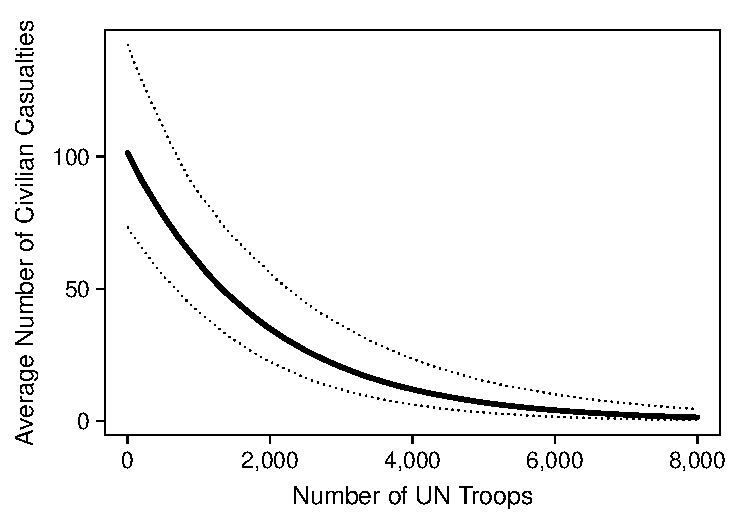
\includegraphics[scale = .8]{figs/hks-ev.pdf}
\caption{This figure shows expected number of civilian casualties as the number of UN troops increases.}\label{fig:hks-ev}
\end{center}
\end{figure}

% Direction
Noting that the relevant coefficients are statistically significant and correctly signed, Hultman, Kathman, and Shannon write:

\begin{quote}
The negative and statistically significant ($p < 0.001$) effects of \textit{UN Military Troops} and \textit{UN Police} suggest that as PKOs are increasingly supplied with soldiers and police forces, violence against civilians in civil war decreases (p. 9-10).
\end{quote}

% Magnitude
The authors argue that effect is not only statistically significant, but substantively important.

\begin{quote}
The figure shows that increasing the number of troops has a \emph{dramatic effect} on improving the safety of noncombatants. With no troops deployed to a conflict, the expected number of civilians killed in a given month is approximately 106. When the number of UN military troops increases to 8,000, the expected value of civilian deaths declines to 1.79. Conditional on the other variables being held at the specified values, supplying only several thousand military troops \emph{nearly mutes} violence completely as the number of troops approaches the upper values reported (p. 11, emphasis ours).
\end{quote}

\noindent They continue:

\begin{quote}
Bear in mind that the values presented are expected civilian deaths per month. These are \emph{not inconsequential} reductions in violence. Indeed, given that the average length of a conflict in these data is nearly 65 months, deploying highly equipped missions can \emph{mitigate or wholly avert humanitarian disasters} (p. 11, emphasis ours).
\end{quote}

% but they fail to take uncertainty into account
Notice that the authors clearly and carefully discuss the substantive importance of their estimated effect--their work serves as an exemplar in this regard. They do not, however, compute a confidence interval around their estimated effect. Thus, they do not consider whether trivial effects are also plausible based on the data. Instead, they only check that the \emph{point estimate} is substantively important. We further their analysis by calculating and interpreting 90\% confidence intervals around the changes in the expected counts.

To assess whether their substantive claim is robust to accounting for the uncertainty, we exactly reproduce their results and calculate the expected changes in civilian deaths as the number of UN military troops increases and 90\% confidence intervals. Figure \ref{fig:hks-ci} shows these estimates and confidence intervals. At an expense of roughly \$2 million, 2,000 troops lead to about 65 fewer civilian casualties, on average. However, the data suggest that the troops lead to \textit{at least} 45 fewer civilian casualties and possibly as many as 95. Similarly, at an expense of about \$8 million, 8,000 troops lead to the prevention of about 100 civilian casualties, but \emph{at least} 70 and perhaps as many as 140. 

\begin{figure}[H]
\begin{center}
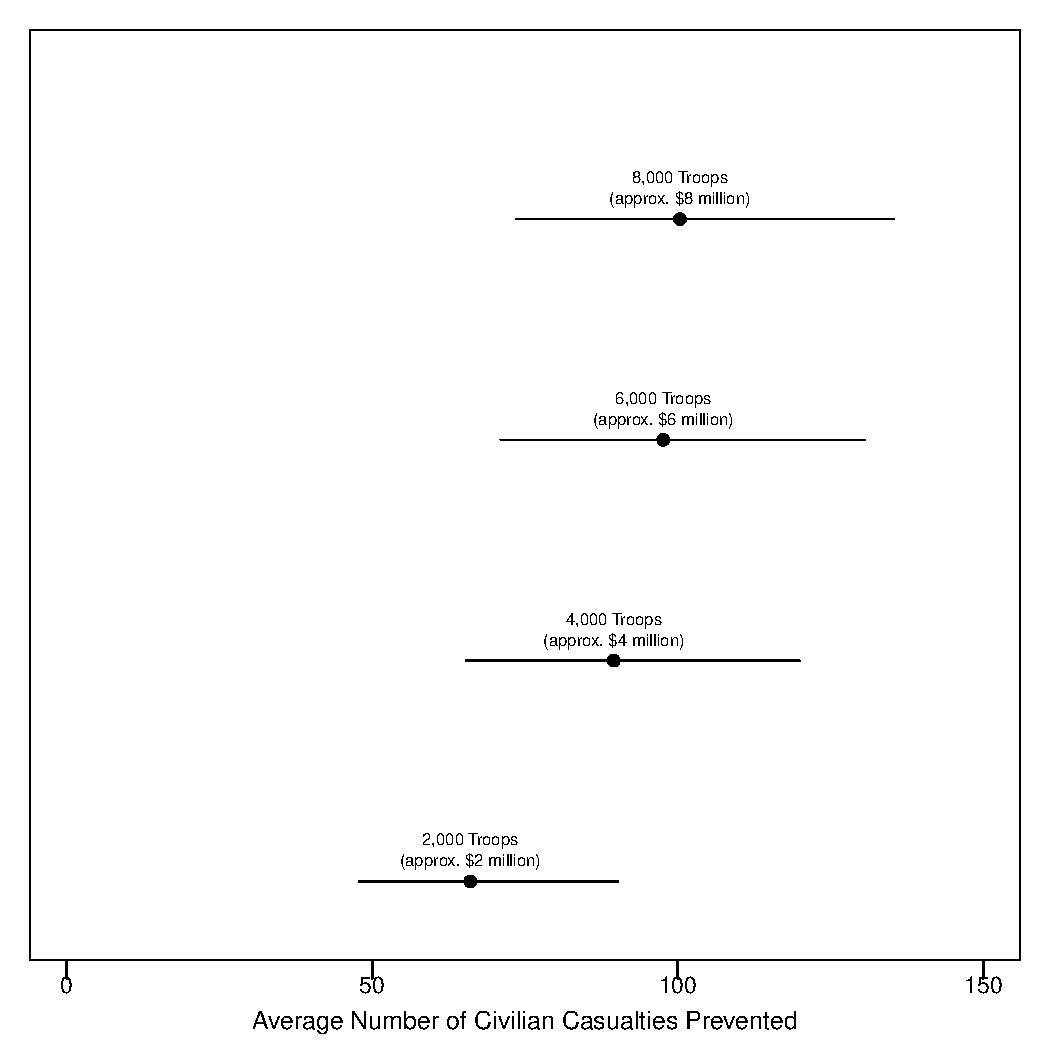
\includegraphics[scale = .8]{figs/hks-ci.pdf}
\caption{This figure provides first differences, in dollar and troop amounts, and their corresponding number of prevented civilian casualties.}\label{fig:hks-ci}
\end{center}
\end{figure}

% summary of our point
In this case, the authors indeed have strong evidence for a \emph{dramatic effect}, even after uncertainty is taken into account. While the data support their claim, the authors can make an even stronger argument for a meaningful effect by substantively interpreting the range of plausible values rather than focusing narrowly on the point estimate. 

\section*{Reanalysis of Kam and Zechmeister (2013)}

% overview of kz
As a second example, we also reanalyze data from \cite{KamZechmeister2013}. Kam and Zechmeister argue that name recognition increases a candidate's support directly, by increasing the candidate's approval, and indirectly, by informing voters about the candidate's viability. The authors present three lab experiments to demonstrate the causal link between their concepts of interest, but they use a field experiment to boost the external validity of the laboratory results and to establish their substantive importance. 

% the basic design
Through a clever design exploiting routes that parents must use to drop their kids off at school, Kam and Zechmeister expose half of parents in a particular geographic region to four yard signs displaying fictitious candidate Ben Griffin's name. The other half of parents are not exposed to any name and serve as a control group. The authors then survey the parents and ask them to indicate their top three choices for city council seats by choosing among five actual candidates and two fictional candidates (Ben Griffin, whose name appeared on yard signs and Milt Jenkins, whose name did not appear on any signs and who serves as a placebo). 

% the basic results
The authors summarize their results:

\begin{quote}
Did recognition spurred on by political yard signs increase support for Ben Griffin in the treatment group? To determine if this is so, we examine the extent to which survey respondents selected Ben Griffin as one of their top three choices for council. As shown in [their] Table 3, in the control condition, only 13.9\% of respondents placed Ben Griffin among their top three choices, but in the treatment condition, 23.9\% of respondents placed Ben Griffin among their top three choices. This 10 percentage point difference is sizable given the modesty of the treatment. In light of the small sample size, it is statistically significant at generous levels ($p \approx 0.13$, one-tailed) (p. 983).
\end{quote}

\noindent They continue:

\begin{quote}
[W]e can examine the rates of selection of the two fictitious names, within each condition. Among the treated subjects, 23.9\% of subjects placed Ben Griffin in the top three set, but only 13.0\% placed Milt Jenkins in the top three set, a statistically significant difference at p < 0.09, one-tailed. Among the control subjects, 13.9\% placed Ben Griffin in the top three set, and the identical percentage, 13.9\%, placed Milt Jenkins in the top three set. The results from this field study lend generalizability to the claim established in our laboratory studies: name recognition increases candidate support in low-information elections (p. 983)
\end{quote}

% are their claims robust to considering uncertainty?
Can we be confident that this effect is indeed ``sizable''? Are small effects plausible given the data? Figure \ref{fig:kz-ci} shows the estimated effects and 90\% confidence intervals. Notice that while the estimated effects are of borderline statistical significance, the estimated effects of about 10 percentage points are quite large. However, much smaller effects are plausible as well. The authors cannot reject even the tiniest of effects with these data. While we agree with the authors that an effect of ten percentage points is indeed ``sizable,'' their data are also consistent with small, negligible effects. As such, these data do not offer compelling evidence for a substantively meaningful effect.

\begin{figure}[H]
\begin{center}
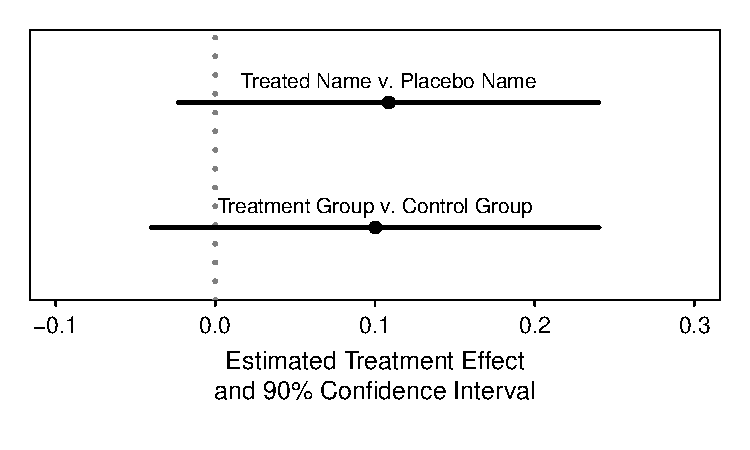
\includegraphics[scale = .8]{figs/kz-ci.pdf}
\caption{This figure provides the estimated treatment effect and 90\% confidence intervals of placing candidate roadsigns along a street that citizens regularly drive on the probability of ranking the named candidate in the top three of seven candidates. The top estimate compares the treatment with the control group (i.e., parents driving along different routes), and the bottom estimate compares the named candidate to the placebo candidate among parents driving along the route with the yard signs.}\label{fig:kz-ci}
\end{center}
\end{figure}

These two examples clearly show that uncertainty in estimated effects matters \textit{substantively}. Researchers should not hide uncertainty behind a veil of statistical significance nor treat uncertainty as a secondary concern. If researchers care about the magnitude of effects, then the range of possibilities should receive as least a much attention as the point estimate.

\subsection*{Conclusion}

In this paper, we argue that researchers should explicitly account for uncertainty when making judgments about the substantive importance of their results. Our suggestion that researchers formally test that effects lie above a threshold of substantive significance is not new (\citealt{Achen1982}, \citealt{Rainey2014a}, and \citealt{Gross2014}; see also \citealt{EsareyDanneman2014}). However, explicit testing of substantive claims is not yet common practice, and scholars rarely offer complete, substantive interpretations of the range of effects contained in their confidence intervals. 

We hope that our discussion encourages researchers to move beyond the current practice and adopt two conventions. First, we recommend that researchers carefully interpret the range of values contained in the confidence intervals. Second, we suggest that researchers avoid making substantive claims based on point estimates when these claims are not also consistent with the range of values contained in the confidence intervals. Using this approach, researchers can (1) compute quantities that are of direct substantive interest, (2) clarify claims about the effects they consider theoretically and/or normatively important, and (3) take the uncertainly of the estimates into account when assessing the evidence for their substantive claims. This leads to more transparent substantive claims and clearer communication of the empirical evidence for these claims.


\singlespace
\bibliographystyle{apsr_fs}
\bibliography{/Users/carlislerainey/Dropbox/papers/bibliography/bibliography.bib}
%\bibliography{/Users/kellymccaskey/Dropbox/Projects/bibliography/bibliography.bib}

\end{document}